\documentclass[9pt,twocolumn]{extarticle}

\usepackage[utf8]{inputenc}
\usepackage{newpxtext} % An improved version of the Palantino font...
\usepackage{newpxmath} % ...and its math version.
\usepackage{authblk}   % Use author blocks.
\usepackage[top=2cm,bottom=2.5cm,left=2cm,right=2cm]{geometry}
\usepackage{balance}
\usepackage{tikz}
\usepackage{xspace} % For reasonable spacing in custom commands.
\usepackage{xcolor} % For colourful links.
\usepackage[backend=biber,style=alphabetic,backref=true,maxnames=20,urldate=long]{biblatex}
\usepackage{hyperref} % For clickable links.
\usepackage[l2tabu, orthodox]{nag}
\usepackage{subcaption}

\setlength{\columnsep}{0.7CM}

\addbibresource{paper.bib}

\definecolor{darkblue}{rgb}{0.1,0.1,0.4}

\newcommand{\ie}{{\it i.e.}\xspace}
\newcommand{\eg}{{\it e.g.}\xspace}
\newcommand{\ea}{{\it et al.}\xspace}
\newcommand{\etc}{{\it etc.}\xspace}
\newcommand{\aka}{a.k.a.\xspace}
\newcommand{\first}{(\emph{i})\xspace}
\newcommand{\second}{(\emph{ii})\xspace}
\newcommand{\third}{(\emph{iii})\xspace}
\newcommand{\fourth}{(\emph{iv})\xspace}
\newcommand{\fifth}{(\emph{v})\xspace}

\hypersetup{
	pdftitle={How do Tor users interact with onion services?},
	pdfauthor={},
	pdfkeywords={},
	colorlinks=true,
	urlcolor=darkblue,
	linkcolor=darkblue,
	citecolor=darkblue
}

\renewcommand*{\bibfont}{\small}

\title{
    {\Huge \textbf{How do Tor users interact with onion services?}}
}

\author{}

\begin{document}

\maketitle

\begin{abstract}
The abstract goes here.
\end{abstract}


\section{Introduction}
\label{sec:introduction}

Online anonymity is typically synonymous with \emph{client anonymity}; VPNs
promise to disguise one's IP address, An equally pressing requirement can be
\emph{server anonymity} when the operator of a site is facing harassment or legal
repercussions.  Decoupling a server's content from the identity of its operator
can mitigate these issues.  Several systems implement various flavours of server
anonymity, including I2P, Freenet, and X, but in this work we focus on Tor's
onion services.

The Tor anonymity network is primarily known as a tool that enables client
anonymity, \ie, it allows users who download the project's Tor Browser to
browse the web anonymously~\cite{Dingledine2004a}.  In addition to client
anonymity, Tor provides server anonymity in the form of onion services (\aka
hidden services) which allow operators to expose a TCP service over the Tor
network while hiding its IP address.

Onion services have grown substantially over the last years, both in the number
of services and users.  As of May 2017, The Tor Project's statistics show that
more than 50,000 onion services are online each day, relaying more than 750 MBps
of network traffic.  Not all of these services host web sites---other use cases
such as meta data-free messaging~\cite{ricochet} and file
sharing~\cite{onionshare} have emerged as well.  Learning the number of onion
service users is more challenging.  In 2016, Facebook reported that more than
one million users logged into their onion service over a one month
period~\cite{facebook-users}.
RFC~\cite{rfc7686}

Past usability research focused on Tor Browser~\cite{Clark2007a,Norcie2014a}
and Tor's censorship circumvention~\cite{Fifield2015a}.  The usability of onion
services remains mostly unexplored.

The most salient aspect of onion services is their peculiar domain names.
Being derived from RSA public keys, they consist of random Base32 characters
such as the following three examples.

{\footnotesize
\begin{verbatim}
6hylx55pr5dnod4t.onion
ke33kjltp3twmcwq.onion
4v4ndsnrjekbfhij.onion
\end{verbatim}
}

Onion domains are random, very difficult to remember, and cumbersome to work
with.  The next generation of onion services exacerbates this problem by
employing domains consisting of 54 (instead of sixteen) Base32-encoded
characters, giving them the following format:

{\footnotesize
\begin{verbatim}
lfels7g3rbceenuuqmpsz45z3lswakqf56n5i3bvqhc22d5rrszzwd.onion
llamanymityx4fi3l6x2gyzmtmgxjyqyorj9qsb5r543izcwymlead.onion
odmmeotgcfx65l5hn6ejkaruvai222vs7o7tmtllszqk5xbysolfdd.onion
\end{verbatim}
}

Properties that we take for granted in the non-onion web are not present in the
onion web.  The usability of onion services differs from ordinary websites in
the following aspects that we are trying to capture in our survey.  The first
issue is \emph{accessibility}.  Onion services are only accessible over Tor for
full client anonymity.\footnote{Services such as Tor2web allow normal web
clients to access onion services but that means that users give up client
anonymity~\cite{tor2web}.} The next issue is onion service \emph{discovery}.
It is difficult to learn about new onion sites.  There is no central directory,
and---unlike the web---onion sites do not link to each other
much~\cite{Griffith2017a}.  However, search engines such as ahmia.fi and
onion.link are a beginning.  Once users learn about new onion service, their
\emph{domain format} makes it difficult to memorize them.  Perhaps the most
salient idiosyncrasy of onion domains is that they are generated randomly.  As
a result, onion domains are difficult to memorize and recognize, forcing users
to handle them differently than normal websites.  Browsing onion sites may feel
clunky because of \emph{latency}---the number of hops in between Tor user and
onion service is causing tangible communication latency that many users may not
be willing to tolerate.

To date, only anecdotal evidence exists on how people interact with onion
services.  In this work we seek to fill this gap by administering a survey
designed to answer the following research questions: \emph{How do Tor users
interact with onion services?}  An answer to this research question allows us
to both create more usable anonymity systems and build these systems in a way
that semantic attacks such as phishing are exacerbated.\footnote{Downs \ea
distinguish between physical (\ie targeting physical infrastructure),
syntactic (\ie targeting software), and semantic (\ie targeting humans)
attacks~\cite[\S~1]{Downs2006a}.}  In particular, we seek to answer the
following three aspects:

%%%
In this paper, we answer our research question by conducting a survey.
We seek to inform X and Y to do Z better.
%%%

\begin{itemize}
    \item What is the expectation of privacy when people use Tor Browser in
        general and onion sites in particular?
    \item What is the security/usability trade-off of vanity onion domains?
    \item Do people handle onion domains differently than normal domains?
\end{itemize}

The rest of this paper is structured as follows.  We begin by discussing related
work in Section~\ref{sec:related-work}, followed by technical background in
Section~\ref{sec:background}.  Section~\ref{sec:survey-design} presents the
design of our survey and Section~\ref{sec:results} analyzes our results.  We
then discuss our results in Section~\ref{sec:discussion} and conclude in
Section~\ref{sec:conclusion}.


\section{Related work}
\label{sec:related-work}

\begin{itemize}
    \item Victors \ea proposed the Onion Name System~\cite{Victors2017a}.
    \item Punycode issues~\cite{Zheng2017a}.  Not a problem for onion services
        since they are all ASCII characters.
    \item Sai and Fink proposed a mnemonic system that maps 80-bit onion domains
        to sentences~\cite{Sai2012a}.  Their work is inspired by mnemonicode, a
        method to map binary data to words~\cite{mnemonicode}.
    \item OpenSSH uses ASCII ``drawings'' to illustrate
        fingerprints~\cite{Loss2009a}.
    \item Kadianakis discussed ways that would make next-generation onion
        domains easier to work with~\cite{Kadianakis2017a}.
    \item Filast{\`o} and Appelbaum proposed a petname system for Tor2Web,
        allowing onion service operators to register
        mnemonics~\cite{Filasto2011a}.
    \item Plasmoid showed how users can be tricked into accepting malicious
        fingerprints, exploiting that most people only look at the first and
        last couple of digits~\cite{Plasmoid2003a}.
    \item Tan \ea looked at how different fingerprint comparison mechanisms
        fare~\cite{Tan2017a}.
    \item Namecoin is technology built on top of Bitcoin that implements a
        generic key $\rightarrow$ value mapping mechanism.  It can serve as a
        DNS replacement, but suffers from poor usability~\cite{Kalodner2015a}.
    \item Hash visualization~\cite{Perrig1999a,Dhamija2005a}.
    \item Bonneau and Schechter showed how 56-bit secrets can be stored in
        ``human memory''~\cite{Bonneau2014a}.
    \item Susceptibility to phishing~\cite{Downs2006a,Sheng2010a}.
    \item Some work on collaboration practices~\cite{Forte2017a}.

    % 2007
    \item Clark, van Oorschot and Adams used cognitive walkthroughs to study
        how users install, configure, and run Tor~\cite{Clark2007a}.  The
        authors uncovered several usability hurdles such as jargon-laden
        documentation, confusing menus, and insufficient visual feedback.  As
        of May 2017, the study is ten years old---Tor Browser has since seen
        radical changes.

    % 2014
    \item Norcie \ea identified stop-points in the installation and use
        of the Tor Browser Bundle~\cite{Norcie2014a}.\footnote{The Tor Browser
        Bundle was later rebranded and is now known as Tor Browser.}  These
        stop-points represent places in a user interface that require action
        but are met with confusion by users.  Having identified these stop
        points, the authors then issued interface design recommendations and
        subsequently tested these recommendations in a user study.

    % 2015
    \item Motivated by Tor's anti-censorship components, Fifield \ea published
        a design to study the usability of Tor as a censorship circumvention
        tool~\cite{Fifield2015a}.  The authors plan to recruit hundreds of
        users to study how they use Tor's configuration wizard in an
        adversarial setting.  This effort made use of both qualitative and
        quantitative methods, Lee \ea~\cite{Lee2017a} studied the usability of
        Tor Launcher, the graphical configuration tool that allows users to
        configure Tor Browser.  Their results paint a bleak picture; 79\% of
        users' connection attempts in a simulated censored environment failed.
        However, the researchers' showed that their interface improvements
        resulted in less difficulties for users.

    % 2017
    \item Forte \ea studied the privacy practices of contributors to open
        collaboration projects~\cite{Forte2017a}.  The authors interviewed 23
        contributors to The Tor Project and Wikipedia to learn about how
        privacy concerns affect their contribution practices.  The study found
        that contributors worry about an array of threats, including
        surveillance, violence, harrassment, and loss of opporunity.

\end{itemize}

We hope that our results generalize to other systems that use
self-authenticating names such as Freenet~\cite{Freenet} and Bitcoin addresses.


\section{Background}
\label{sec:background}

To create an onion domain, a Tor client first generates an RSA key pair.  It
then computes the SHA-1 hash over the onion service's public key, truncates it
to 80 bits, and encodes these 80 bits in Base32, resulting in sixteen
characters.  Onion domains are self-authenticating, meaning that as long as a
client has the correct domain, it knows what public key to expect.

The perfect naming scheme should have three properties:
\begin{description}
    \item[Secure] The mapping from the name to the underlying resource (e.g., an
        IP address) must be secure.
    \item[Memorable] People should be able to remember the name easily.
    \item[Global] The name should have the same meaning for every participant
        in the system.
\end{description}

\begin{figure}
  \centering

  \begin{subfigure}[b]{\linewidth}
    \centering
    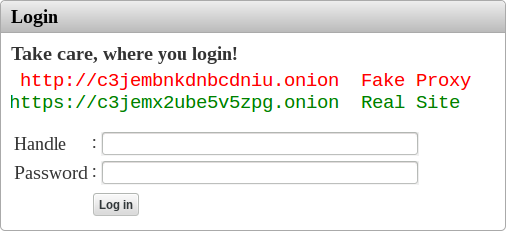
\includegraphics[width=0.7\linewidth]{figures/login-warning-1.png}
    \caption{During the login process, an onion site explicitly warns of an
    impersonation site.}
    \label{fig:login-warning-1}
  \end{subfigure}

  \begin{subfigure}[b]{\linewidth}
    \centering
    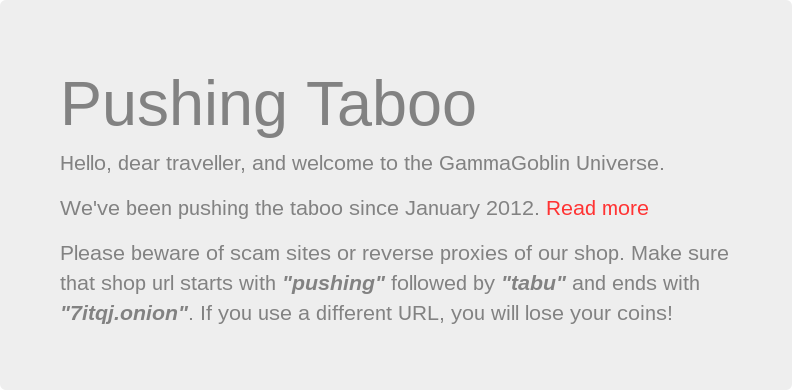
\includegraphics[width=0.8\linewidth]{figures/login-warning-2.png}
    \caption{Aware of an ongoing phishing attack, another onion site warns its
    users of impersonation sites.}
    \label{fig:login-warning-2}
  \end{subfigure}

  \caption{Reacting to phishing attacks, some onion service operators now
  display warnings as part of the login process.}
\end{figure}

Possible to use scallion~\cite{scallion}.

In practice, most naming schemes only seem to satisfy two out of these three
properties.  This observation is colloquially referred to as ``Zooko's
triangle,'' illustrated in \autoref{fig:naming-triangle}.  DNS is memorable
and global but not secure because numerous attacks exist to feed DNS users a
false mapping from domain to IP address.  Onion domains are secure and global
but not memorable because they are long and randomly generated.  Petname systems
(e.g., your buddy list in your instant messaging application) are memorable and
secure but not global.

\begin{figure}
\centering
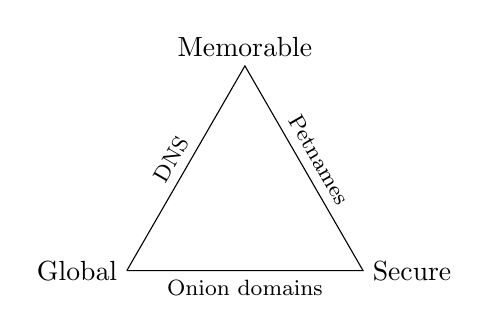
\begin{tikzpicture}

\draw (0.0,0.0) node[anchor=east] {Global}
        -- node [midway, below, sloped] {{\footnotesize Onion domains}}
      (3.0,0.0) node[anchor=west] {Secure}
        -- node [midway, above, sloped] {{\footnotesize Petnames}}
      (1.5,2.6) node[anchor=south] {Memorable}
        -- node [midway, above, sloped] {{\footnotesize DNS}}
      (0.0,0.0);

\end{tikzpicture}
\caption{``Zooko's triangle,'' a conjecture that posits that any naming scheme
can only satisfy two properties out of secure, memorable, and global.}
\label{fig:naming-triangle}
\end{figure}


\section{Survey design}
\label{sec:survey-design}

We investigate how Tor users interact with onion services by designing and
administering a survey.

\subsection{Research question}
We designed the survey to answer the following research questions: \emph{How do
Tor users interact with onion services?}  An answer to this research question
allows us to both create more usable anonymity systems and build these systems
in a way that human-centered attacks such as phishing are exacerbated.  In
particular, we seek to answer the following three aspects:

\begin{itemize}
    \item What is the expectation of privacy when people use Tor Browser in
        general and onion sites in particular?
    \item What is the security/usability trade-off of vanity onion domains?
    \item Do people handle onion domains differently than normal domains?
\end{itemize}

\subsection{Design}
\begin{itemize}
    \item Our survey consists of six blocks:
        \begin{enumerate}
            \item Consent and demographics
            \item Tor usage
            \item Onion site usage
            \item Onion site operation
            \item Onion site phishing and impersonation
            \item Expectations of privacy
        \end{enumerate}
    \item Mention that we got IRB approval once we got it.
    \item We implemented our survey in Qualtrics and made sure that it can be
        answered correctly over Tor Browser.  Used a Qualtrics feature so that
        participants can answer the survey only once.
    \item We used four screener questions distributed over four distinct
        blocks, \ie, questions whose sole purpose is to check whether the
        respondent is paying attention.~\cite{Berinsky2014a}.
    \item Having followed mailing lists \etc for many years, we did not feel the
        need for focus groups to explore what topics are worth inquiring.
    \item Used cognitive pretesting (sometimes also called cognitive
        interviewing)~\cite{Collins2003a}.  Pretesting can show us that
        respondents \first understand questions, \second understand questions
        consistently, and \third understand questions the way that we intended.
        Two main strategies are \emph{think-aloud interviewing} and
        \emph{probing}.  In addition, we can ask respondends about the
        confidence they have in their responses.  However, not all cognitive
        processes can be verbalized and cognitive pretesting may change the way
        respondents answer questions.  We had $N$ respondents (talk about
        demographics) based on whose input we iteratively improved our survey.

        $M$ respondents were fluent, but non-native English speakers.
    \item We tried hard to have neutral, non-leading questions.
    \item Question randomization.
    \item Basic statistics.  The survey consists of X questions and takes
        approximately Y minutes to complete.  We used our university's
        Qualtrics membership to create the survey.
\end{itemize}

\subsection{Participant recruiting}
\begin{itemize}
    \item Tor's population is unknown.  We barely know its size.  Besides, there
        is no way to recruit all Tor users with equal probability.  Therefore,
        we will have inevitable sampling bias in our results.  We work around
        that by using diverse recruitment media and making our sample size as
        large as possible.
    \item Post on Tor's blog?\\\url{https://blog.torproject.org}
    \item Ask Tor to post on its Twitter account?\\\url{https://twitter.com/torproject}
    \item Post on Tor's mailing lists
    \item Post on social media such as:
        \begin{itemize}
            \item \url{https://reddit.com/r/tor/}
            \item \url{https://reddit.com/r/onions/}
            \item \url{https://reddit.com/r/samplesize/}
        \end{itemize}
    \item Use Amazon's Mechanical Turk
    \item Facebook ads?
    \item Google surveys?
    \item Craigslist?
\end{itemize}

Important things to consider in questions:
\begin{itemize}
    \item Are our results generalizable to self-authenticating names?
    \item Ordering of questions matters.
    \item Use aided recall for behavioral questions.
    \item Questions should be non-threatening (is there a ``right'' or ``wrong''
        answer?).  If respondents think they would
        look bad, they may answer not truthfully.
    \item Avoid jargon and unusual vocabulary (to non-native English speakers)
\end{itemize}

\subsection{Incentives for participation}
\begin{itemize}
    \item Have a few high-value gift cards in lottery.
    \item Have many low-value gift cards for everyone.
    \item Bitcoins?
\end{itemize}

\subsection{Data analysis}

\subsection{Limitations}
\begin{itemize}
    \item Representative sample?
\end{itemize}


\section{Results}
\label{sec:results}

\subsection{Participants}
\begin{itemize}
    \item Provide intuition on how much our sample resembles the general
        population.
    \item From when to when did we disseminate our survey?
    \item How many participants did we attract?
    \item How long did it take to complete the survey?  Provide some descriptive statistics.
    \item What's the female/male ratio?
    \item What's the age distribution?
    \item What's the level of education?
    \item What's the computer security knowledge?  Note that our participants
        may overestimate their knowledge.
\end{itemize}

\subsection{Random anecdotes}
\begin{itemize}
    \item In pre-test: one person considered the onion domain itself
        confidential and was worried about the domain's prefix revealing
        anything about its content.
\end{itemize}


\section{Discussion}
\label{sec:discussion}

\begin{itemize}
    \item Tor is working on a new onion service design~\cite{Mathewson2013a}.
        Anything we can say about that?
\end{itemize}

\subsection{Limitations}
\begin{itemize}
    \item Our demographic may not be representative because we selected people
        who may care more about onion sites than the average Tor user.  Many
        Tor users may do nothing other than download Tor Browser.
    \item Our survey was only in English, so it may not generalize well to
        non-English speakers.  We know that there are cultural differences in
        security behavior~\cite{Sawaya2017a}.
\end{itemize}


\section{Conclusion}
\label{sec:conclusion}


\section*{Acknowledgements}
We want to thank George Kadianakis for helpful feedback.

We want to thank Laura M. Roberts, Roya Ensafi, Will Scott, and Jens Kubiziel
for help with pre-testing the survey.

Thanks to Katherine Haenschen for helping us improve our method.

This research was supported in part by the Center for Information Technology
Policy at Princeton University.  This project was further supported in part by
National Science Foundation Awards CNS-1540055 and CNS-1602399.


\balance
\printbibliography

\end{document}
